\documentclass[11pt,letterpaper]{article}

\usepackage{textcomp,marvosym}
\usepackage{amsmath,amssymb}
\usepackage[left]{lineno}
\usepackage{changepage}
\usepackage{rotating}
\usepackage{natbib}
\usepackage{setspace}
\usepackage{fancyhdr}
\usepackage{graphicx}
\usepackage[aboveskip=1pt,labelfont=bf,labelsep=period,justification=raggedright,singlelinecheck=off]{caption}
%\doublespacing

\raggedright
\textwidth = 6.5 in
\textheight = 8.25 in
\oddsidemargin = 0.0 in
\evensidemargin = 0.0 in
\topmargin = 0.0 in
\headheight = 0.0 in
\headsep = 0.5 in
\parskip = 0.1 in
\parindent = 0.2in

\renewcommand{\thefigure}{S\arabic{figure}}

\begin{document}

\begin{flushleft}
{\Large \textbf{Supporting information for ``Primary and secondary red bed magnetization constrained by fluvial intraclasts''}}

\end{flushleft}

\section*{Additional study location information}
The study site in the Freda Formation along the Bad River is within the Ashland Syncline (47.3867\textdegree N, 90.6371\textdegree W, WGS84; Fig. \ref{fig:location_figure}). These outcrop exposures along the Bad River are very fresh as the soil-rock interface dates to retreat from the last glacial maximum which is constrained locally to be 13.2 $\pm$ 0.4 thousand years ago based on nearby $^{10}$Be exposure dates \citep{Ullman2015a}. The outcrops have subsequently been exposed through ongoing river incision (Fig. \ref{fig:location_figure}C). The rocks are very well-preserved for their antiquity. In contrast to localities $\sim$90 km to the east in the White Pine region, there is a lack of mineralization in the underlying Nonesuch Formation in this region \citep{Stewart2017a}. 

\begin{figure}[!ht]
\noindent\includegraphics[width=0.9\textwidth]{location_figure.pdf}
\caption{\small{Geological maps of the study region highlighting bedrock units associated with the Midcontinent Rift. The intraclast study location (47.3867\textdegree N, 90.6371\textdegree W, WGS84) is shown as a red star on the Lake Superior region overview map (A), the zoom-in map of the eastern Ashland syncline (B) and the Bad River (C) for which the geology is overlain on air photo imagery (ESRI World Imagery). CHC stands for Copper Harbor Conglomerate. The geologic map data have been modified from \cite{Survey2011a}, \cite{Nicholson2004a}, and \cite{Jirsa2011a}.}}
\label{fig:location_figure}
\end{figure} 

\section*{Additional details concerning sampling and preparation methods}

Figure \ref{fig:prep_figure} depicts intraclast BRIC-6 in outcrop, drill core and in the lab with the sandstone matrix removed.

\begin{figure}[!ht]
\noindent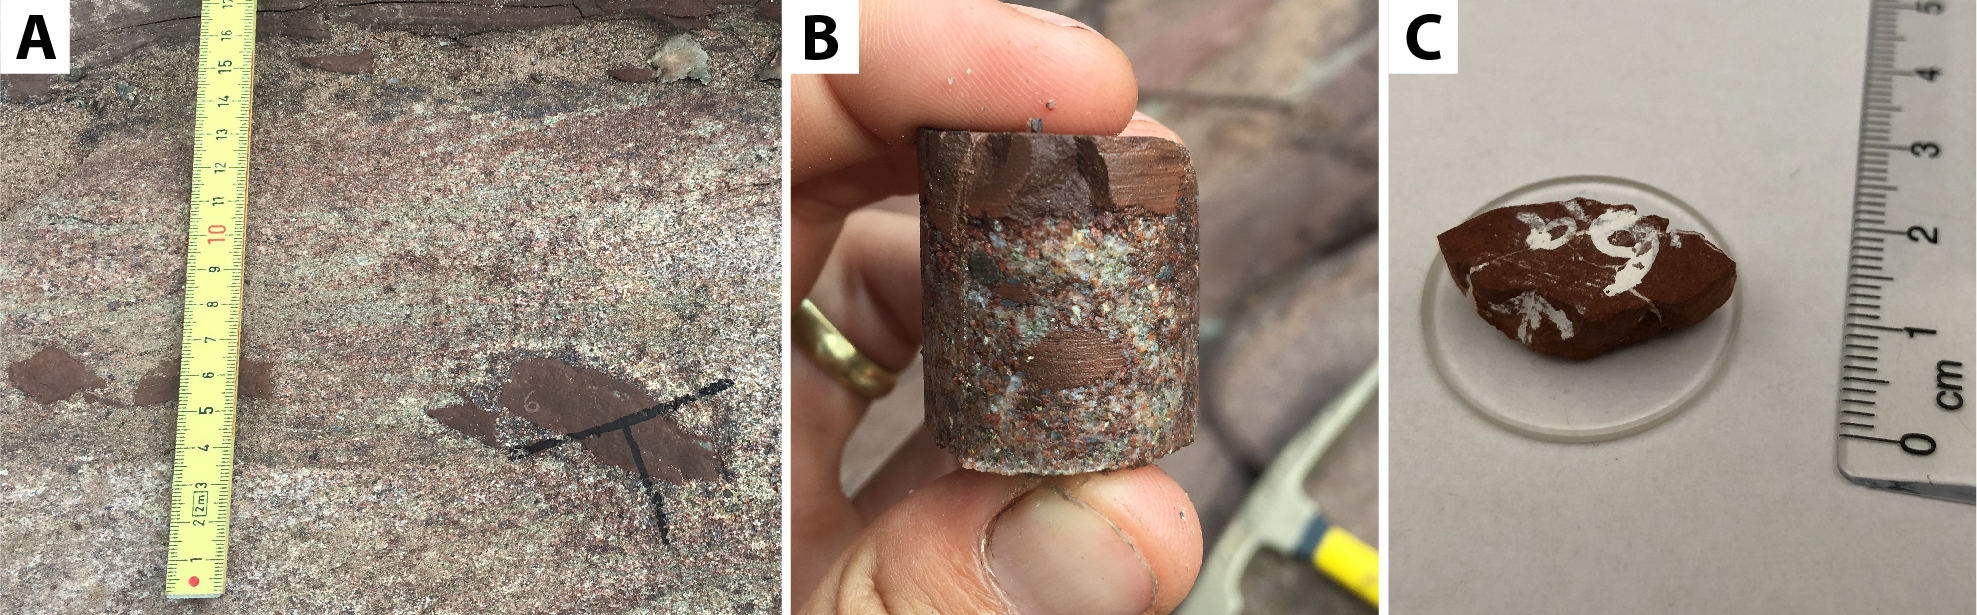
\includegraphics[width=\textwidth]{prep_figure.jpg}
\caption{\small{Photos of intraclast BRIC-6: in the field within coarse sandstone (A), at the top of an oriented drill core sample (B) and prepped with the matrix sandstone removed on a quartz glass disk (C). The numbered divisions on the rulers in A and C are both in centimeters. Panel A shows multiple siltstone intraclasts. The one marked with the $\lambda$ is the clast sampled as BRIC-6.}}
\label{fig:prep_figure}
\end{figure} 

\section*{Additional details concerning petrographic methods}
Microscopic observations were made using a Zeiss EVO-LS10 scanning electron microscope (SEM) in the Energy Geosciences Division of Lawrence Berkeley National Laboratory. This instrument has a paired Oxford Instruments X-Max X-ray energy dispersive spectrometer (EDS) that was used to estimate elemental abundance at submicron-sized spots at specified points and in a mapped grid (Fig. \ref{fig:sem_images}). Within the Department of Earth and Planetary Science at UC Berkeley, a Zeiss EVO-10 Variable Vacuum SEM with paired electron backscatter diffraction (EBSD) detector was used to collect EBSD patterns for targeted grains (Fig. \ref{fig:sem_images}). These EBSD patterns were fit to a catalog of silicate and oxide minerals using OIM Analysis software.

\begin{figure}[!ht]
\centering
\noindent\includegraphics[width=6.2in]{Repository_Image_Figure.png}
\caption{\small{Scanning electron microscopy images and data for sample BRIC-26. The energy-dispersive X-ray spectroscopy (EDS) map shows the distribution of Fe and Ti for the same view as the backscatter image. This map reveals both micron-scale oxide grains (hematite, ilmenite and TiO$_2$) and disseminated iron within clays and the matrix. EDS spectrum are shown for individual labeled grains as are electron backscatter diffraction (EBSD) images matched with the hematite pattern which identifies the grains. These techniques, along with optical reflected light microscopy, were used to identify the grains labeled as hematite in Figure 1 of the main text.}}
\label{fig:sem_images}
\end{figure} 

The mineralogical interpretations based on the petrographic data articulated in the main text, including a predominance of hematite and an overall lack of magnetite among the oxide grains, are consistent with those of \cite{Vincenz1968b} on samples from the Freda Formation. Additional Fe-Ti oxides in the intraclasts were identified as rutile and ilmenite. Some of the hematite grains retain primary exsolution textures consistent with an igneous origin rather than having formed \textit{in situ} as authigenic grains. Petrographic work on the underlying Copper Harbor Formation identified hematite grains on the scale of 10s of microns, but concluded that it was ambiguous whether these grains were detrital or authigenic \citep{Elmore1982a}. The dispersion of the paleomagnetic component that is held by such large grains in the Freda intraclasts strongly supports that, in the case of the Freda siltstones, these grains are detrital.

\bibliographystyle{gsabull}
\bibliography{../../../../0000_Github/references/allrefs}

\end{document}
